\documentclass{standalone}
\usepackage{tikz}
\usetikzlibrary{patterns, positioning}


\begin{document}
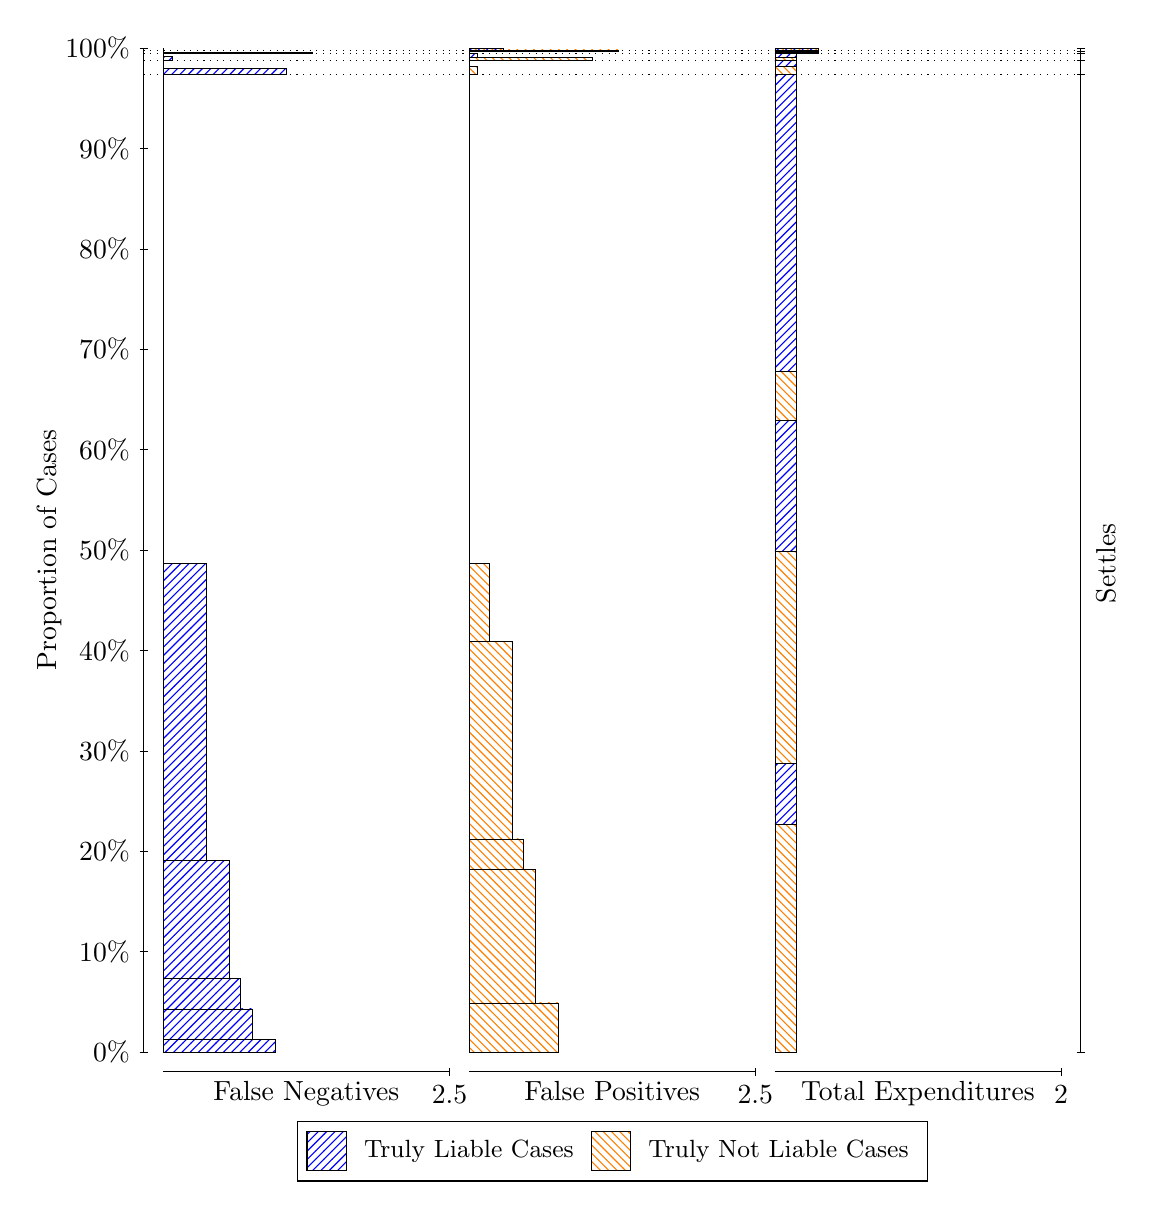
\begin{tikzpicture}
\draw[black, very thin] (1.5,1.75) -- (1.5,14.5);
\node[rotate=90, text=black, anchor=center] at (0.3, 8.125) {Proportion of Cases};
\draw[black, very thin] (1.45,1.75) -- (1.55,1.75);
\node[text=black, anchor=east] at (1.45, 1.75) {0\%};
\draw[black, very thin] (1.45,3.025) -- (1.55,3.025);
\node[text=black, anchor=east] at (1.45, 3.025) {10\%};
\draw[black, very thin] (1.45,4.3) -- (1.55,4.3);
\node[text=black, anchor=east] at (1.45, 4.3) {20\%};
\draw[black, very thin] (1.45,5.575) -- (1.55,5.575);
\node[text=black, anchor=east] at (1.45, 5.575) {30\%};
\draw[black, very thin] (1.45,6.85) -- (1.55,6.85);
\node[text=black, anchor=east] at (1.45, 6.85) {40\%};
\draw[black, very thin] (1.45,8.125) -- (1.55,8.125);
\node[text=black, anchor=east] at (1.45, 8.125) {50\%};
\draw[black, very thin] (1.45,9.4) -- (1.55,9.4);
\node[text=black, anchor=east] at (1.45, 9.4) {60\%};
\draw[black, very thin] (1.45,10.675) -- (1.55,10.675);
\node[text=black, anchor=east] at (1.45, 10.675) {70\%};
\draw[black, very thin] (1.45,11.95) -- (1.55,11.95);
\node[text=black, anchor=east] at (1.45, 11.95) {80\%};
\draw[black, very thin] (1.45,13.225) -- (1.55,13.225);
\node[text=black, anchor=east] at (1.45, 13.225) {90\%};
\draw[black, very thin] (1.45,14.5) -- (1.55,14.5);
\node[text=black, anchor=east] at (1.45, 14.5) {100\%};

\draw[black, very thin] (13.4,1.75) -- (13.4,14.5);
\draw[black, very thin] (13.35,1.75) -- (13.45,1.75);
\node[anchor=west] at (13.35, 1.75) {};
\draw[black, very thin] (13.35,14.164) -- (13.45,14.164);
\node[anchor=west] at (13.35, 14.164) {};
\draw[black, very thin] (13.35,14.339) -- (13.45,14.339);
\node[anchor=west] at (13.35, 14.339) {};
\draw[black, very thin] (13.35,14.432) -- (13.45,14.432);
\node[anchor=west] at (13.35, 14.432) {};
\draw[black, very thin] (13.35,14.464) -- (13.45,14.464);
\node[anchor=west] at (13.35, 14.464) {};
\draw[black, very thin] (13.35,14.5) -- (13.45,14.5);
\node[anchor=west] at (13.35, 14.5) {};

\draw[black, very thin, pattern color=blue, pattern=north east lines] (1.75,1.75) rectangle (3.167,1.9088);
\draw[black, very thin, pattern color=blue, pattern=north east lines] (1.75,1.9088) rectangle (2.8763,2.2976);
\draw[black, very thin, pattern color=blue, pattern=north east lines] (1.75,2.2976) rectangle (2.731,2.681);
\draw[black, very thin, pattern color=blue, pattern=north east lines] (1.75,2.681) rectangle (2.5857,4.1876);
\draw[black, very thin, pattern color=blue, pattern=north east lines] (1.75,4.1876) rectangle (2.295,7.9591);
\draw[black, very thin, pattern color=orange, pattern=north west lines] (1.75,7.9591) rectangle (1.75,14.164);
\draw[black, very thin, pattern color=blue, pattern=north east lines] (1.75,14.164) rectangle (3.3123,14.24);
\draw[black, very thin, pattern color=orange, pattern=north west lines] (1.75,14.24) rectangle (1.75,14.339);
\draw[black, very thin, pattern color=blue, pattern=north east lines] (1.75,14.339) rectangle (1.859,14.393);
\draw[black, very thin, pattern color=orange, pattern=north west lines] (1.75,14.393) rectangle (1.75,14.432);
\draw[black, very thin, pattern color=blue, pattern=north east lines] (1.75,14.432) rectangle (3.6393,14.444);
\draw[black, very thin, pattern color=orange, pattern=north west lines] (1.75,14.444) rectangle (1.75,14.464);
\draw[black, very thin, pattern color=orange, pattern=north west lines] (1.75,14.464) rectangle (1.75,14.475);
\draw[black, very thin, pattern color=blue, pattern=north east lines] (1.75,14.475) rectangle (1.75,14.5);
\draw[black, very thin, pattern color=orange, pattern=north west lines] (5.6333,1.75) rectangle (6.7597,2.3736);
\draw[black, very thin, pattern color=orange, pattern=north west lines] (5.6333,2.3736) rectangle (6.469,4.0726);
\draw[black, very thin, pattern color=orange, pattern=north west lines] (5.6333,4.0726) rectangle (6.3237,4.4561);
\draw[black, very thin, pattern color=orange, pattern=north west lines] (5.6333,4.4561) rectangle (6.1783,6.963);
\draw[black, very thin, pattern color=orange, pattern=north west lines] (5.6333,6.963) rectangle (5.8877,7.9547);
\draw[black, very thin, pattern color=blue, pattern=north east lines] (5.6333,7.9547) rectangle (5.6333,14.164);
\draw[black, very thin, pattern color=orange, pattern=north west lines] (5.6333,14.164) rectangle (5.7423,14.263);
\draw[black, very thin, pattern color=blue, pattern=north east lines] (5.6333,14.263) rectangle (5.6333,14.339);
\draw[black, very thin, pattern color=orange, pattern=north west lines] (5.6333,14.339) rectangle (7.1957,14.379);
\draw[black, very thin, pattern color=blue, pattern=north east lines] (5.6333,14.379) rectangle (5.7423,14.432);
\draw[black, very thin, pattern color=orange, pattern=north west lines] (5.6333,14.432) rectangle (5.6333,14.452);
\draw[black, very thin, pattern color=blue, pattern=north east lines] (5.6333,14.452) rectangle (5.6333,14.464);
\draw[black, very thin, pattern color=orange, pattern=north west lines] (5.6333,14.464) rectangle (7.5227,14.475);
\draw[black, very thin, pattern color=blue, pattern=north east lines] (5.6333,14.475) rectangle (6.0693,14.5);
\draw[black, very thin, pattern color=orange, pattern=north west lines] (9.5167,1.75) rectangle (9.7892,4.6404);
\draw[black, very thin, pattern color=blue, pattern=north east lines] (9.5167,4.6404) rectangle (9.7892,5.4126);
\draw[black, very thin, pattern color=orange, pattern=north west lines] (9.5167,5.4126) rectangle (9.7892,8.1034);
\draw[black, very thin, pattern color=blue, pattern=north east lines] (9.5167,8.1034) rectangle (9.7892,9.7688);
\draw[black, very thin, pattern color=orange, pattern=north west lines] (9.5167,9.7688) rectangle (9.7892,10.392);
\draw[black, very thin, pattern color=blue, pattern=north east lines] (9.5167,10.392) rectangle (9.7892,14.164);
\draw[black, very thin, pattern color=orange, pattern=north west lines] (9.5167,14.164) rectangle (9.7892,14.263);
\draw[black, very thin, pattern color=blue, pattern=north east lines] (9.5167,14.263) rectangle (9.7892,14.339);
\draw[black, very thin, pattern color=orange, pattern=north west lines] (9.5167,14.339) rectangle (9.7892,14.379);
\draw[black, very thin, pattern color=blue, pattern=north east lines] (9.5167,14.379) rectangle (9.7892,14.432);
\draw[black, very thin, pattern color=orange, pattern=north west lines] (9.5167,14.432) rectangle (10.062,14.452);
\draw[black, very thin, pattern color=blue, pattern=north east lines] (9.5167,14.452) rectangle (10.062,14.464);
\draw[black, very thin, pattern color=orange, pattern=north west lines] (9.5167,14.464) rectangle (10.062,14.475);
\draw[black, very thin, pattern color=blue, pattern=north east lines] (9.5167,14.475) rectangle (10.062,14.5);
\draw[black, dotted] (1.5,14.164) -- (13.4,14.164);
\draw[black, dotted] (1.5,14.339) -- (13.4,14.339);
\draw[black, dotted] (1.5,14.432) -- (13.4,14.432);
\draw[black, dotted] (1.5,14.464) -- (13.4,14.464);
\draw[black, very thin] (1.75,1.5) -- (5.3833,1.5);
\node[text=black, anchor=north] at (3.5667, 1.5) {False Negatives};
\draw[black, very thin] (5.3833,1.45) -- (5.3833,1.55);
\node[text=black, anchor=north] at (5.3833, 1.45) {2.5};

\draw[black, very thin] (5.6333,1.5) -- (9.2667,1.5);
\node[text=black, anchor=north] at (7.45, 1.5) {False Positives};
\draw[black, very thin] (9.2667,1.45) -- (9.2667,1.55);
\node[text=black, anchor=north] at (9.2667, 1.45) {2.5};

\draw[black, very thin] (9.5167,1.5) -- (13.15,1.5);
\node[text=black, anchor=north] at (11.333, 1.5) {Total Expenditures};
\draw[black, very thin] (13.15,1.45) -- (13.15,1.55);
\node[text=black, anchor=north] at (13.15, 1.45) {2};

\node[text=black, centered, rotate=90] at (13.72, 7.9569) {Settles};





\draw (7.449999999999999,1.5) node[draw=none] (baseCoordinate) {};
\begin{scope}[align=center]
        \matrix[scale=0.5, draw=black, below=0.5cm of baseCoordinate, nodes={draw}, column sep=0.1cm]{
            \node[rectangle, draw, minimum width=0.5cm, minimum height=0.5cm, pattern color=blue, pattern=north east lines] {}; &
            \node[draw=none, font=\small, text=black] (B) {Truly Liable Cases}; &
            \node[rectangle, draw, minimum width=0.5cm, minimum height=0.5cm, pattern color=orange, pattern=north west lines] {}; &
            \node[draw=none, font=\small, text=black] (B) {Truly Not Liable Cases}; \\
            };
\end{scope}

\end{tikzpicture}
\end{document}